\graphicspath{{figures/chap02/}}

%\chapter{等离子体原子发射谱线与碰撞辐射模型}
\chapter{原子谱线强度比诊断等离子体电子温度与密度概述}
\label{chap:crm-intro}

不同元素原子的能级结构是不相同的,具有不同的光谱辐射。通过对原子发射光谱的测量和分析,不仅可以定性地分析气体成分,还可以定量地分析各种元素的含量。根据不同原子受激发以及发射光谱的难易程度还可以进行等离子参数的诊断测量,例如电子温度 $T_{\rm e}$ 和电子密度 $N_{\rm e}$。

\section{原子谱线强度比诊断电子温度与密度}

原子受到激发后,由高能级 $j$ 跃迁到低能级 $i$ 时,将辐射出一定能量的光子,光子的波长 $\lambda_{ji}$ 由能级间的能量差 $\Delta E$ 决定:
\begin{equation}
  \lambda_{ji} = \frac{h{\rm c}}{\Delta E}
\end{equation}
式中,$h$ 为普朗克常数(Planck Constant),${\rm c}$ 为光速。其光子数辐射率可以写为\cite{Wiese1966:book}:
\begin{equation}
  %\label{}
  \epsilon_{ji}=\frac{1}{4\pi}N_{j}A_{ji}
\end{equation}
其中,$N_j$ 为跃迁上能级 $j$ 的粒子数密度,$A_{ji}$ 为自发辐射跃迁速率系数(爱因斯坦系数)。

假设均匀等离子体条件下,光谱测量系统获得的光子辐射计数率 $I_{\lambda_{ji}}$ 为:
\begin{equation}
  I_{\lambda_{ji}}=\epsilon_{ji}V\Omega T_{\lambda_{ji}}\eta_{\lambda_{ji}}
\end{equation}
其中,$V$ 为光谱仪可观测到的等离子体体积,$\Omega$ 为光谱接收设备所呈的立体角,$T_{\lambda_{ji}}$ 为等离子体的透射率,$\eta_{\lambda_{ji}}$ 为光学探测系统的量子效率。如果同时测量另外一条波长为 $\lambda_{qp}$ 的谱线,则两条谱线的强度比:
\begin{equation}
\label{eq:chap02:line-ratio}
  \frac{I_{\lambda_{ji}}}{I_{\lambda_{qp}}}=
  \frac{\epsilon_{ji}T_{\lambda_{ji}}\eta_{\lambda_{ji}}}{\epsilon_{qp}T_{\lambda_{qp}}\eta_{\lambda_{qp}}}
  =\frac{1}{F_R}\frac{T_{\lambda_{ji}}N_jA_{ji}}{T_{\lambda_{qp}}N_qA_{qp}}
\end{equation}
其中,$F_R$ 为与仪器响应相关的系数,实验中可以进行标定;自发辐射跃迁速率系数可以通过理论计算获得精确的数值,且一般不受等离子体参数的影响(第 \ref{sec:chap02:Aji} 节)。而由于跃迁上能级的粒子数密度 $N_{j}$ 与 $N_{q}$ 随电子温度与密度具有不同的变化趋势,这样通过建立反映原子反应过程的模型,事先计算出谱线比(式 \ref{eq:chap02:line-ratio})随等离子体电子温度与密度的变化趋势,在实验中测量出对应谱线的强度比,即可以根据模型计算结果反推出等离子体的电子温度和密度。

以 Z 箍缩氖等离子体中氖原子的 $K$ 壳层谱线辐射为例\cite{LiJing:WLXB},通过建立描述原子反应过程的碰撞辐射模型,计算出 ${\rm H}_\alpha$ 和 ${\rm I.C.}$ 谱线分别与 ${\rm He}_\alpha$ 谱线的强度比在电子温度--电子密度空间内的分布,其等高线如图 \ref{fig:chap02:lijing-a} 与 \ref{fig:chap02:lijing-b} 所示,其中谱线强度比 ${\rm H}_\alpha/{\rm He}_\alpha$ 主要与电子温度相关,谱线强度比 ${\rm I.C.}/{\rm He}_\alpha$ 主要与电子密度相关。如果在实验中同时测量该两谱线强度比值分别为 $0.53$ 与 $0.15$ 时,即可以同时确定等离子体的电子温度与密度参数,如图 \ref{fig:chap02:lijing-c} 所示。

\begin{figure}%[H]
  \centering
  \begin{subfigure}{0.45\textwidth}
  \begin{overpic}[width=\textwidth]{lijing-a.pdf}
    \put(15,63.5){\mbox{\colorbox{white}{\small\hspace{1em}}}}
    %\put(-2,30){\rotatebox{90}{\mbox{\colorbox{white}{\small\hspace{2em}激发截面 (${\rm m}^2$)\hspace{2em}}}}}
  \end{overpic}
  \caption{谱线强度比 ${\rm H}_\alpha/{\rm He}_\alpha$ 等高线}
  \label{fig:chap02:lijing-a}
  \end{subfigure}
  \hspace{0.03\textwidth}
  \begin{subfigure}{0.45\textwidth}
  \begin{overpic}[width=\textwidth]{lijing-b.pdf}
    \put(86,65){\mbox{\colorbox{white}{\hspace{0.5em}}}}
    %\put(-2,25){\rotatebox{90}{\mbox{\colorbox{white}{\small\hspace{2em}激发速率系数 (${\rm m}^3/{\rm s}$)\hspace{2em}}}}}
  \end{overpic}
  \caption{谱线强度比 ${\rm I.C.}/{\rm He}_\alpha$ 等高线}
  \label{fig:chap02:lijing-b}
  \end{subfigure}
  \\%\hspace{0.03\textwidth}
  \begin{subfigure}{0.45\textwidth}
  \begin{overpic}[width=\textwidth]{lijing-c.pdf}
    %\put(30,0){\mbox{\colorbox{white}{\small\hspace{2em}$T_{\rm e} (${\rm eV}$)$\hspace{2em}}}}
    %\put(-2,25){\rotatebox{90}{\mbox{\colorbox{white}{\small\hspace{2em}激发速率系数 (${\rm m}^3/{\rm s}$)\hspace{2em}}}}}
  \end{overpic}
  \caption{同时确定电子温度和密度的关系曲线}
  \label{fig:chap02:lijing-c}
  \end{subfigure}
  \caption{Z 箍缩氖等离子体中氖 $K$ 壳层的 ${\rm H}_\alpha$ 和 ${\rm I.C.}$ 与 ${\rm He}_\alpha$ 谱线的强度比的模型计算等高线(图 \ref{fig:chap02:lijing-a} 与 \ref{fig:chap02:lijing-b})与两谱线强度比分别为 $0.53$ 和 $0.15$ 时同时确定电子温度与密度的关系曲线(图 \ref{fig:chap02:lijing-c})。图片来自 \onlinecite{LiJing:WLXB}。}
  \label{fig:chap02:lijing}
\end{figure}

%\section{原子发射谱线}
\section{影响原子发射谱线强度的过程}

理论上要计算有多少光子辐射出等离子体区域,需要对以下三个过程进行分析:1)原子激发态自发辐射跃迁几率;2)特定的等离子体条件下原子激发态数密度;3)光子在等离子体中的传播。

\subsection{自发辐射跃迁几率}
\label{sec:chap02:Aji}

自发辐射跃迁几率可以通过原子物理相关理论计算获得,不同的等离子体环境(如温度、密度等)会对原子状态产生影响,但一般来讲等离子体环境对原子激发态自发辐射跃迁几率的影响微乎其微,可以忽略。$j\to i$ 自发辐射跃迁速率系数 $A_{ji}$ 可以由以下方程给出\cite{Kolb1964:A-formular}:
\begin{equation}
  A_{ji}=4.3\times10^7\frac{g_i}{g_j}f_{ij}\Delta E_{ji}^2\,{\rm s}^{-1}
\end{equation}
其中,$g_i$、$g_j$ 和 $\Delta E_{ji}$ 分别为 $i$、$j$ 能级的统计权重和两能级能量差,$f_{ij}$ 为 $i$ 到 $j$ 能级的吸收振子强度(absorption oscillator strength)\cite{Johnson1972:collisionalstrength}。另外,自发辐射跃迁系数也可以在数据库\cite{NISTdatabase}中直接查询获得。

\subsection{描述原子激发态数密度分布的模型}

%现阶段,爱因斯坦系数可以精确获得。而
式 (\ref{eq:chap02:line-ratio}) 中上能级的粒子数 $N_j$ 与 $N_q$ 与等离子体电子温度 $T_{\rm e}$ 和 $N_{\rm e}$ 相关。通过建立原子反应过程模型,事先计算等离子体辐射谱线上能级的粒子数密度与 $T_{\rm e}$ 和 $N_{\rm e}$ 的关系,则可通过测量谱线的强度比反推等离子体的电子温度和密度。

在特定的 $T_{\rm e}$ 和 $N_{\rm e}$ 参数下,通过对等离子体内影响特定原子激发态数密度的反应过程进行研究,以确定此激发态的数密度。这些原子反应过程一般为\cite{atomicprocesses,YuChangxuan:book}:

\begin{enumerate}
  \item 辐射跃迁
    \begin{itemize}
      \item 同步辐射跃迁(spontaneous radiative decay)
      \item 辐射复合(radiative recombination)
      \item 自发电离(autoionization)
      \item 双电子复合(dielectronic capture)
    \end{itemize}
  \item 自由电子碰撞
    \begin{itemize}
      \item 激发(excitation)
      \item 退激发(deexcitation)
      \item 电离(ionization)
      \item 复合(recombination)
    \end{itemize}
  \item 光致过程
    \begin{itemize}
      \item 光致激发(photoexcitation)
      \item 光致退激发(photodeexcitation)
      \item 光致电离(photoionization)
      \item 光致辐射复合(induced radiative recombination)
    \end{itemize}
  \item 重粒子碰撞
    \begin{itemize}
      \item 激发(excitation)
      \item 退激发(deexcitation)
      \item 电离(ionization)
      \item 电荷交换(charge exchange)
    \end{itemize}
\end{enumerate}

原则上,将这些过程的反应速率方程一一列出,并联立求解这些方程即可得到等离子体内各粒子的数密度。

但等离子体中包含了大量的粒子和数目巨大的相互碰撞反应过程,实际工作中不可能将所有反应过程进行描述并求解。实际的研究工作中,人们一般根据等离子体密度高低将等离子体分为三种模型进行描述:日冕模型、碰撞辐射模型和局域热平衡模型。图 \ref{fig:chap02:plasma_model_region} 所示为以拥有三个能级(基态和两个激发态能级)的原子为例,将三种模型的反应过程图像进行示意。

\begin{figure}%[H]
  \centering
  \begin{overpic}[width=0.9\textwidth]{plasma_model_region_used.pdf}
    \put(4,1){\mbox{\colorbox{white}{\hspace{2em}日冕图像\hspace{2em}}}}
    \put(36,1){\mbox{\colorbox{white}{\hspace{2em}碰撞辐射图像\hspace{2em}}}}
    \put(69,1){\mbox{\colorbox{white}{\hspace{2em}局域热平衡图像\hspace{2em}}}}
  \end{overpic}
  %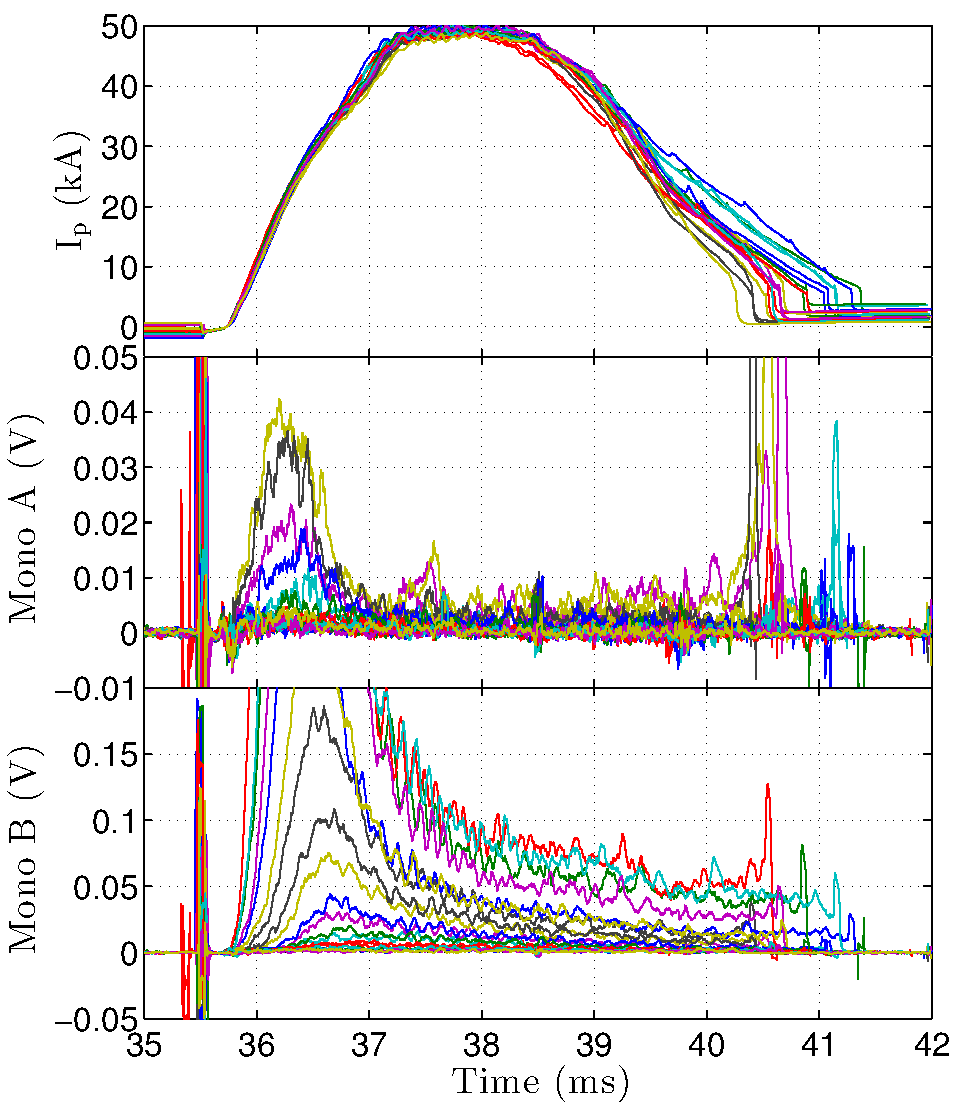
\includegraphics[width=0.7\textwidth]{AH72_BH32.pdf}
  \caption{具有三个能级(基态和两个激发态)原子的日冕图像、碰撞辐射图像和局域热平衡图像示意图。图片来自\onlinecite{Menhart2000:Thesis}。}
  \label{fig:chap02:plasma_model_region}
\end{figure}

\emph{日冕模型}\quad 在低密度等离子体($n<10^{11}\,{\rm cm}^{-3}$)中,等离子体内原子激发态的自发辐射跃迁几率远高于其碰撞损失过程(激发/退激发)的跃迁几率。所以,模型中仅考虑基态的碰撞激发、电离以及激发态的自发辐射跃迁过程。此时,激发态能级粒子的数密度要远低于基态能级的粒子数密度。

\emph{碰撞辐射模型}\quad 当等离子体密度较高时,碰撞过程反应速率增加。此时原子激发态数密度由碰撞和自发辐射过程的相互竞争决定。在碰撞辐射图像中,激发态原子的激发、退激发和电离过程等反应开始变得重要。托卡马克聚变等离子体的密度处在 $10^{11}\,{\rm cm}^{-3}\sim 10^{16}\,{\rm cm}^{-3}$ 区间,其原子反应过程应使用碰撞辐射模型描述。

\emph{局域热平衡模型}\quad 当等离子体密度高于 $10^{18}\,{\rm cm}^{-3}$ 时,碰撞反应过程的速率进一步加大,甚至超过自发辐射跃迁过程,此时激发态原子的自发辐射跃迁过程可以忽略。此时,原子激发态与基态之间处于局域热平衡状态。原子激发态之间和电离态之间的粒子数密度分布分别为麦克斯韦分布和萨哈分布,其分布函数可在 \onlinecite{YuChangxuan:book} 中找到。

\subsection{谱线辐射在等离子体内的传播}

激发态自发辐射跃迁产生的光子在等离子体的传播过程一般需要复杂的辐射输运方程进行描述\cite{Holstein1947:PhysRev.72.1212,Holstein1951:PhysRev.83.1159,Phelps1958:PhysRev.110.1362}。
实际计算中,人们一般采取简化的处理方法,如使用光学厚度和逃逸因子描述等离子体对光子辐射的吸收\cite{Johnson1972:collisionalstrength,boivin2001}。

其中,光学逃逸因子 $\Lambda$(optical escape factor)表示可以逃离等离子体区域的光子与总辐射光子的比例,逃逸因子接近或等于 $1$ 时,等离子体即为光性薄的。平均光学厚度 $\tau_0$(mean optical depth)为等离子体对光谱的指数吸收因子($I=I_0{\rm e}^{-\tau_0}$),当 $\tau_0\le0.01$ 时,对应的等离子体为光性薄的。

%要对逃逸因子和光学厚度进行计算,需要针对每条谱线辐射列出响应的辐射和吸收输运方程。
对于氦等离子体,如果谱线的多普勒展宽为主要展宽机制时\cite{Wiese1966:book},平均光学厚度和光学逃跑因子可以用下列公式计算\cite{Drawin1973:OEF,boivin2001}:
\begin{align}
  \tau_0&=\frac{n_ig_jA_{ji}\lambda_{ji,0}^3r}{8g_i\pi^{3/2}v_{\rm th}} \label{eq:chap02:mod}\\
  \Lambda&=1-\left(\frac{\tau_0}{\sqrt{2}}-\frac{\tau_0^2}{2!\sqrt{3}}+\frac{\tau_0^3}{3!\sqrt{4}}\cdots\frac{(-1)^{n+1}\tau_0^n}{n!\sqrt{n+1}}\right)
\end{align}
其中,$n_i$ 为跃迁低能级的粒子数密度,$g_j$ 和 $g_i$ 分别为跃迁对应高能级和低能级的统计权重,$\lambda_{ji,0}$ 为谱线的中心波长,$v_{\rm th}$ 为氦原子的热速度,$r$ 为等离子体特征尺度(半径)。另外,当谱线的主要展宽机制为非多普勒展宽时,J. He 等人\cite{HeJian2006:ef}计算了氦谱线辐射为洛仑兹(Lorentzian)和沃伊特(Voigt)线形时的逃逸因子。

\section{碰撞辐射模型}

%\subsection{原子反应速率方程}
托卡马克等离子体中的原子反应过程一般由碰撞辐射模型描述,对于等离子体内的某电离态离子的激发态能级粒子 $p$,其数密度 $N_p$ 随时间的变化由下面的速率方程决定:
\begin{equation}
\begin{aligned}
  \frac{{\rm d}N_p}{{\rm d}t}=
  &-\left\{\sum_{q\ne p}C_{pq}N_{\rm e}+\sum_{q<p}A_{pq}+S_{p\nu}N_{\rm e}+r_{p\mu}N_{\rm e}\right\}N_p\\
  &+\left\{\sum_{q\ne p}C_{qp}N_q+\sum_{q>p}A_{qp}N_q\right\}+\left\{S_{\mu p}N_{\mu}+r_{\nu p}N_\nu\right\}N_{\rm e}
\end{aligned}
\end{equation}
其中,$C$、$A$、$S$、$r$ 和 $N$ 分别表示电子碰撞激发或退激发速率系数、自发辐射跃迁几率、电子碰撞电离速率系数、电子碰撞复合速率系数和粒子数密度;下标中 $q$、$\mu$、$\nu$ 和 ${\rm e}$ 分别表示与 $p$ 能级具有相同电离态的 $q$ 激发态能级离子(或原子,下同)、低电离态离子、高电离态离子和电子。可见,对于 $p$ 能级粒子,其主要损失过程包括电子碰撞激发或退激发、电离和复合以及自发辐射跃迁过程;其产生过程也类似地由这些过程决定。

将等离子体内此电离态的基态和亚稳态粒子记为 $\rho$(在碰撞辐射模型中,亚稳态与其他普通激发态粒子的处理没有本质不同,其特性由原子反应过程的速率系数体现),其他激发态粒子记为 $i$,高电离态离子记为 $\nu$,低电离态粒子记为 $\mu$。对每个粒子的数密度 $N$ 列出其速率方程,即可得以下完备的粒子反应速率方程\cite{Summers2006}:
\begin{equation}
\label{eq:chap02:gcr}
\frac{{\rm d}}{{\rm d}t}
\begin{bmatrix}N_\mu\\ N_\rho\\ N_i\\ N_\nu\end{bmatrix}
=
\begin{bmatrix}
	\mathcal{C}_{\mu'} 	& N_{\rm e}\mathcal{R}_{\rho'\mu} & 0 & 0 \\
	N_{\rm e}\mathcal{S}_{\mu'\rho} & \mathcal{C}_{\rho'} & \mathcal{C}_{i'\rho} & N_e\mathcal{R}_{\nu'\rho} \\
	0 & \mathcal{C}_{\rho'i} & \mathcal{C}_{i'} & N_{\rm e}\mathcal{R}_{\nu'i} \\
	0 & N_{\rm e}\mathcal{S}_{\rho'\nu} & N_{\rm e}\mathcal{S}_{i'\nu} & \mathcal{C}_{\nu'}
\end{bmatrix}
\begin{bmatrix}
	N_{\mu'}\\ N_{\rho'}\\ N_{i'}\\ N_{\nu'}
\end{bmatrix}
\end{equation}
其中,方程右侧第一项碰撞辐射矩阵中,$\mathcal{S}$ 与 $\mathcal{R}$ 分别为离子的电离和复合速率系数向量。非对角元素 $\mathcal{C}$ 表示电子碰撞激发/退激发和自发辐射跃迁速率系数向量,以 $\mathcal{C}_{\rho'i}$ 为例:
\begin{equation}
  \mathcal{C}_{\rho'i}=\sum_{\rho'\ne i}C_{\rho'i}N_{\rm e}+\sum_{\rho'>i}A_{\rho'i}
\end{equation}
对角元素表示此粒子的总损失速率,以 $\mathcal{C}_{\rho'}$ 为例:
\begin{equation}
  \mathcal{C}_{\rho'}=-\left\{\left(\mathcal{R}_{\rho'\mu}+\mathcal{S}_{\rho'\nu}\right)N_{\rm e}+\mathcal{C}_{\rho'i}\right\}
\end{equation}
另外,粒子上标 $'$ 表示上一时刻的粒子数密度。

方程 (\ref{eq:chap02:gcr}) 描述了等离子体内各能级粒子(离子)的数密度随时间的变化。其中包含了两个假设:1)模型中只包含只有一个电子得失的电离和复合过程;2)电离和复合过程的产物粒子只处于基态或亚稳态。通过求解此方程可以获得随时间的演化情况,也可以计算系统达到稳态时的结果。对于达到平衡的磁约束聚变等离子体而言,等离子体中粒子碰撞和辐射跃迁过程的时间常数远小于等离子体的粒子约束时间,人们一般采用反应速率方程达到稳态时的计算结果。

%\section{前人在氦原子碰撞辐射模型研究中存在的问题}
\section{氦原子碰撞辐射模型在诊断应用中存在的问题}
\label{sec:chap02:crm-problem}
%\subsection{}

在利用氦原子谱线比诊断托卡马克等离子体 $T_{\rm e}$ 和 $N_{\rm e}$ 的研究中,为了得到更高精度的计算结果,人们不断尝试改进原子反应速率系数的精度,并增加在碰撞辐射模型中包含的能级粒子、反应过程以及可以对原子能级产生影响的因素。但因为使用的截面数据精度不一,导致碰撞辐射模型中包含更多的能级和反应过程时,并不能如预期那样获得更高精度的计算结果(图 \ref{fig:chap02:lineratio-compare-n3})。
%人们不断尝试改进原子反应速率系数的精度,并增加在碰撞辐射模型中包含的能级粒子,以期得到更高精度的激发态粒子数密度计算结果。

\begin{figure}%[H]
  \centering
  \begin{overpic}[width=\textwidth]{lineratio-compare-n3-black.pdf}
  \end{overpic}
  \caption{不同碰撞辐射模型计算的来自 $n=3$ 壳层的谱线比结果对比。(a):$T_{\rm e}=20\,{\rm eV}$ 时,$N_{\rm e}$ 敏感谱线比 $I_{667.8}/I_{728.1}$ 的对比;(b):$N_{\rm e}=1.0\times10^{12}\,{\rm cm}^{-3}$ 时,$T_{\rm e}$ 敏感谱线比 $I_{728.1}/I_{706.7}$ 的对比。模型和数据来源:Schweer1992:来自 \onlinecite{Schweer1992174} ($n\le4$);NIFS($n\le4$):来自 \onlinecite{Sasaki:NIFS:DATA:049};NIFS($n\le20$):来自 \onlinecite{Sasaki:NIFS:DATA:049};Kubo1999:来自 \onlinecite{Hirotaka1999-HeCRM-JT60U},使用 \onlinecite{Fujimoto1979-HeCR} 的模型;Ma2012:来自 \onlinecite{MaShuiliang2012:Tomography},使用 \onlinecite{Goto2003-HeCRM} 的模型;Burgos2012:来自 \onlinecite{burgos2012:PoP};CRM:本文碰撞辐射模型。}
  \label{fig:chap02:lineratio-compare-n3}
\end{figure}


1)原子反应速率系数不确定性

原子反应速率系数(或截面)数据主要有以下三种来源:实验测量
\cite{Shah1988:ionizaiton-data-measure,Long1970:PhysRevA.1.260,Dixon1976}、
理论计算\cite{CCCmethod,Sawey199381}与半经验公式拟合\cite{Fujimoto:IPPJ-AM-8},并且有人对此专门做过总结
\cite{IAEA:Data:vol3,deHeer:INDC,Kato:NIFS:DATA:346}。图 \ref{fig:chap02:xsec-compare} 所示为不同数据来源的电子碰撞激发和速率系数的对比。在碰撞辐射模型方面,人们也在一直将最新的速率系数总结结果应用在计算中,例如,M. Goto\cite{Goto2003-HeCRM} 将以前的碰撞辐射模型\cite{Fujimoto1979-HeCR} 使用的反应速率系数数据进行了更新。然而这些数据来源的精度难以保证\cite{Ralchenko2008603},导致不同来源原子反应数据的碰撞辐射其计算结果也不尽相同\cite{Delabie2010:consistency}。%如第 \ref{sec:chap01:research-history} 节所述,

碰撞辐射模型中包含着数目巨大的激发态能级和复杂的相关反应过程,且各粒子之间通过原子反应相互关联。目前并没有有效的手段可以对速率系数不确定性至激发态数密度计算误差之间的传递进行计算。Y. Andrew 等人\cite{Andrew2000PPCFSensitivity}提出了一种计算方法,在假设碰撞辐射模型中某一过程的速率系数具有不确定性时,对此速率系数进行干扰,并重新求解碰撞辐射模型,以获得该速率系数的不确定性对粒子数密度计算的影响。通过对所有的速率系数进行干扰并重新求解碰撞辐射模型,即可得到模型中各反应过程速率系数的影响。这种方法并不直观,速率系数不确定性至激发态数密度计算误差传递之间的物理意义不明确,且每次都要对碰撞辐射模型进行重新求解,也不能对速率系数精度提出具体的要求。

\begin{figure}%[H]
  \centering
  \begin{subfigure}{0.45\textwidth}
  \begin{overpic}[width=\textwidth]{meta-exc-xsec-compare.pdf}
    \put(30,0){\mbox{\colorbox{white}{\small\hspace{2em}$T_{\rm e} (${\rm eV}$)$\hspace{2em}}}}
    \put(-2,30){\rotatebox{90}{\mbox{\colorbox{white}{\small\hspace{2em}激发截面 (${\rm m}^2$)\hspace{2em}}}}}
  \end{overpic}
  \caption{电子碰撞激发 $2^3{\rm S}\to 3^3{\rm D}$ 的截面}
  \label{fig:chap02:xsec-compare-meta}
  \end{subfigure}
  \hspace{0.03\textwidth}
  \begin{subfigure}{0.45\textwidth}
  \begin{overpic}[width=\textwidth]{l-change-exc-rate-compare.pdf}
    \put(30,0){\mbox{\colorbox{white}{\small\hspace{2em}$T_{\rm e} (${\rm eV}$)$\hspace{2em}}}}
    \put(-2,25){\rotatebox{90}{\mbox{\colorbox{white}{\small\hspace{2em}激发速率系数 (${\rm m}^3/{\rm s}$)\hspace{2em}}}}}
  \end{overpic}
  \caption{电子碰撞激发 $3^3{\rm S}\to 3^3{\rm P}$ 的速率系数}
  \label{fig:chap02:xsec-compare-l-change}
  \end{subfigure}
  \caption{不同数据来源的电子碰撞激发和速率系数数据对比。图片来自
  \onlinecite{Goto1997-HeCRM-WT3},数据来源详见 \onlinecite{Goto1997-HeCRM-WT3} 的参考文献。}
  \label{fig:chap02:xsec-compare}
\end{figure}

2)模型中包含的激发态能级和反应过程

最早人们使用最高包含至 $n=4$ 壳层的碰撞辐射模型\cite{Brosda1993:Thesis,Schweer1992174},后来在模型中增加了 $5\le n\le9$ 的激发态和 ${\rm He}^+$\cite{Schmitz2008},随着模型的发展,包含了越来越多的能级\cite{Ahn2007-He-BES},甚至最高包含到了 $n=500$ 壳层的能级\cite{burgos2012:PoP}。然而,通过将这些模型谱线比的计算结果进行对比(图 \ref{fig:chap02:lineratio-compare-n3})发现,这些模型并没有因为包含了跟多的能级和反应过程而获得高精度的结果。

首先,对于很高激发态的能级,现阶段无法对其电子碰撞激发或电离的截面进行精确的理论计算,实验更是无法进行测量。模型中,只能通过经验上的定标关系来计算,然而这种定标关系的精度是很难保证的。其次,对于高激发态能级,其粒子数密度会急剧减少\cite{Fujimoto1979-HeCR,Griem1964-book},然而在模型中使用低精度的反应截面数据将其包含在计算中,这不但不会带来更高精度的计算结果,反而可能会带来更大的计算误差。目前,在使用相同的速率系数的前提下,在模型中包含不同的能级和反应过程对计算结果影响的研究还鲜有报道。其中,文献  \onlinecite{Sasaki:NIFS:DATA:049} 中给出了模型包含 $n\le4$ 和 $n\le20$ 时不同的计算结果,但没有详细分析模型中包含不同能级粒子时,计算结果将会呈现什么样的趋势。


\section{小结}

本章首先介绍了可同时诊断等离子体电子温度与密度的原子谱线辐射强度比法,然后从光子产生到被光谱测量设备探测接收所经历的物理过程出发,给出影响谱线强度的因素,包括:自发辐射跃迁几率、光子在等离子体内传播过程中的再吸收和激发态粒子数密度。其中,自发辐射跃迁几率系数可以获得高精度的数据,对于光性薄的等离子体,激发态粒子数密度与其电子密度和电子温度参数相关,通过建立描述等离子体内各粒子的原子反应速率方程,即可以求解出在不同的等离子体参数情况下的激发态粒子数密度。通过实验测量来自不同激发态的谱线,根据其谱线强度比,既可以反推出等离子体的电子温度和密度参数。

在实际研究中,人们根据等离子体密度的不同对等离子体内的反应过程进行不同的简化。对高温聚变等离子体,需要使用碰撞辐射模型以计入原子碰撞激发/退激发、电离/复合以及自发辐射跃迁等过程,以求解激发态粒子数密度。然而,原子反应过程速率系数(截面)数据的精度受到很大限制,以致人们在模型中包含越来越多的能级粒子和反应过程,却不能如预期的那样得到更高精度的结果。同时,由于碰撞辐射模型中包含了数目巨大的能级粒子和复杂的反应过程,目前并无有效手段对速率系数不确定性至能级粒子数密度计算误差的传递进行直接的有效计算。一般使用对速率系数进行干扰并再次求解模型的速率方程的方法,这种分析手段并不直观,也不易操作,对不确定性的传递也不能给出明确的物理意义。

